\documentclass[12pt]{amsart}
\usepackage{geometry} % see geometry.pdf on how to lay out the page. There's lots.
\usepackage{graphicx}
\geometry{a4paper} % or letter or a5paper or ... etc
% \geometry{landscape} % rotated page geometry

% See the ``Article customise'' template for come common customisations

\title{PINT white paper}
\author{Jing Luo et. al}
\date{1/21/2014} % delete this line to display the current date

%%% BEGIN DOCUMENT
\begin{document}

\maketitle
\tableofcontents

\section{Introduction}
(Introduction of pulsar timing) \\
We have developed a new timing package/library, named PINT, which is tempo/tempo2 independent. The new package differs from tempo in many essential respects from the structure to coding. (1) Using the well-debugged libraries and strong isolated modulars for the flexibility of future development and user customizing. (2) Coding in Python and taking full advantage of self-describing objects and python standard library. (3) Well defined interface and GUI will not be required. (4) Well documented by docstrings. \\
The library structure will be described in section 2.(More coming)
\section{Structure}
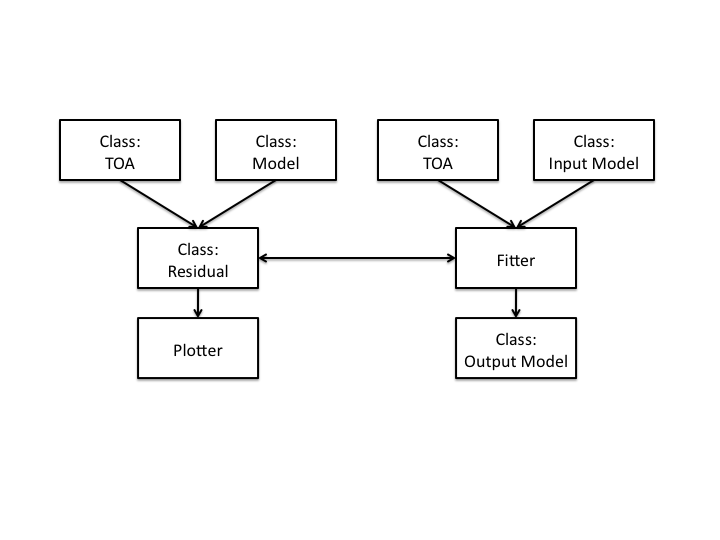
\includegraphics[width=\textwidth]{PINTflow_chart.png}
\end{document}